% !TeX root = ../main.tex

\section{Proposed Project and Innovation}
\subsection*{System and User Workflow}

\textbf{Project Goals.} Our project aims to investigate \textbf{what makes an argument persuasive} and whether certain writing techniques are more effective depending on topic and conversational context. We want explore questions such as: 

\begin{enumerate}
    \item Are certain rhetorical strategies more effective for particular topics?
    \item Does participating in a longer discussion with multiple comments increase the likelihood of changing someone's opinion?
    \item Are polite, well-structured arguments more persuasive than confrontational ones? 
    \item How do appeals to ethos (credibility), pathos (emotion), and logos (logic) influence an argument's effectiveness?
\end{enumerate}

By analyzing these elements, we hope to identify patterns that help explain why some arguments successfully change people's minds while other don't. Ultimately, our goal is not simply to predict if an argument is persuasive, but to help users understand why certain arguments may be more effective than others and how rhetorical choices interact with context.

\textbf{Project Artifacts.} Our working artifact will be an interactive ML-powered argument analysis and visualization tool, intended for writers, students, researchers, and individuals seeking to improve the persuasiveness in their writing. 

The system will accept a written argument as text (or document upload), with a short form to collect information about the intended topic, audience, and additional context. It will combine multiple pretrained and potentially fine-tuned machine learning models to predict and explain the argument's persuasiveness. 

Rather than providing only a single persuasiveness score, the system will visually decompose the argument into meaningful components. For example, it may: 

\begin{enumerate}
    \item \textbf{Identify rhetorical appeals:} Highlight passages that employ ethos, pathos, or logos.
    \item \textbf{Evaluate argument quality:} Estimate characteristics such as logical coherence, clarity, evidence use, politeness, and argument development.
    \item \textbf{Predict persuasiveness:} Estimate how persuasive the argument is based on patterns learned from annotated datasets.
    \item \textbf{Visualize the argument's structure: }Show how different rhetorical strategies and writing characteristics are distributed throughout the text.
    \item \textbf{Provide contextual feedback:} Explore whether specific techniques are more effective for the selected topic or intended audience, where supported by the available data.
    \item \textbf{Grammar:} Are arguments more persuasive if grammar score is higher?
\end{enumerate}

\begin{figure}
    \centering
    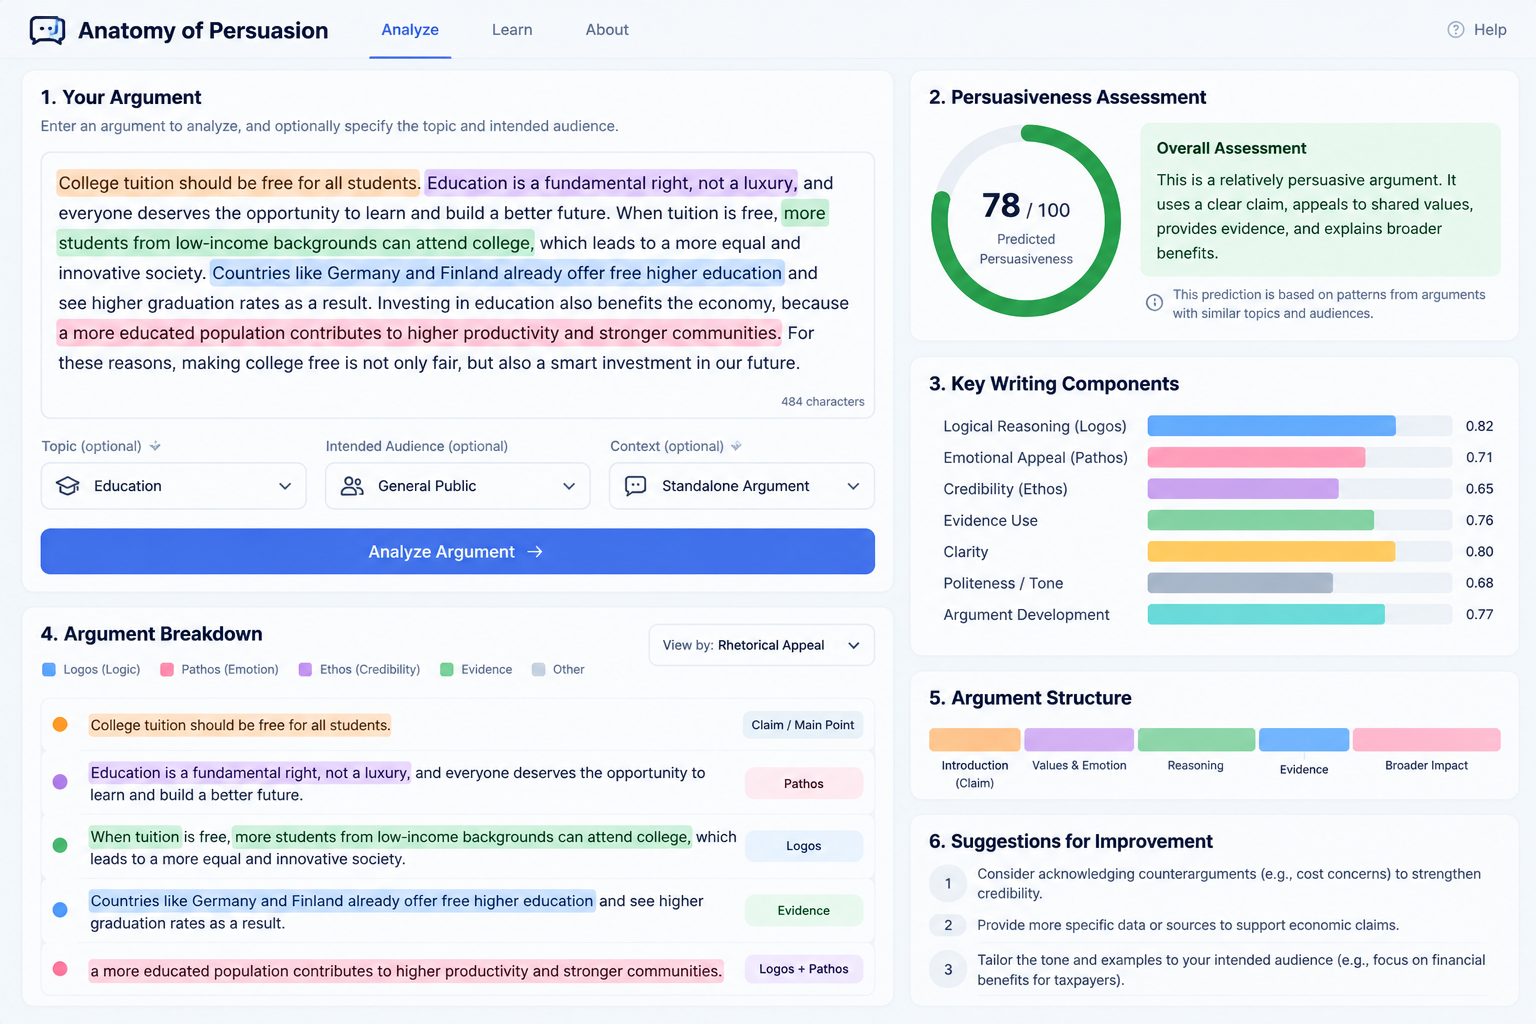
\includegraphics[width=0.75\linewidth]{proposal/figures/visual-idea.png}
    \caption{Proposed interface for visualizing argument persuasiveness, rhetorical strategies, writing components, and ML-generated feedback.}
    \label{fig:placeholder}
\end{figure}

\textbf{Approach.} Our initial approach will use existing pretrained models, supplemented by models fine-tuned by our team on argument quality, rhetorical strategy, grammar analysis, and persuasion datasets where appropriate. We may also investigate combining predictions from multiple specialized models into a unified assessment. The primary end-to-end task is to allow a user to submit an argument and receive an interpretable visual breakdown of its persuasive characteristics, along with a predicted persuasiveness assessment and explanations of the features contributing to that prediction.

\subsection*{Connection Between Visualization and Machine Learning}


\subsection*{Innovation and Comparison With Existing Work}
\textbf{Closest existing approach.}
\todo{Name and cite the closest system or method. Describe how it would handle the same task and where the proposed workflow differs.}

\textbf{Expected contribution.}
Our proposed contribution is \todo{a precise design, method, adaptation, or empirical finding}, distinguished by \todo{one or two concrete differences}.
We will assess its value by \todo{comparison that tests those differences}.
\todo{Explain why the contribution is useful even if the underlying ML algorithm is established. Avoid claiming novelty without checking the literature.}

\textbf{Minimum deliverable and optional extension.}
\todo{Define a working core with one dataset, one ML method, and the essential views/interactions. Identify one optional extension to attempt only after the core and evaluation work.}
